\documentclass{article}

\title{Complex Analysis Homework, Section 10}
\author{Adam Buskirk}

\usepackage{amssymb,amsmath,amsthm}
\usepackage{tikz}
\usepackage[margin=1in]{geometry}

\newtheorem{theorem}[subsection]{Theorem}
\newtheorem{conjecture}[subsection]{Conjecture}
\newtheorem{lemma}[subsection]{Lemma}
\theoremstyle{definition}
\newtheorem{definition}[subsection]{Definition}

\newcommand{\R}{\mathbb{R}}
\newcommand{\N}{\mathbb{N}}
\newcommand{\Q}{\mathbb{Q}}
\newcommand{\Z}{\mathbb{Z}}
\newcommand{\Co}{\mathbb{C}}
\newcommand{\p}[1]{\left(#1\right)}
\newcommand{\sq}[1]{\left[#1\right]}
\newcommand{\set}[1]{\left\{#1\right\}}
% \newcommand{\p}[1]{\left(#1\right)}

\begin{document}
\maketitle

\section{Problem 10.3.a}
The roots will be
\[ z = 1 \exp \sq{i\p{ \frac{\pi+2k\pi}{3} }}, \qquad k=0,1,2 \]
Which yields roots $(\cos(\frac{\pi}{3}),\sin(\frac{\pi}{3}))=\frac{1}{2}+i\frac{\sqrt{3}}{2}$
(for $k=0$),
$-1$ (for $k=1$),
and $\frac{1}{2}-i\frac{\sqrt{3}}{2}$ (for $k=2$).

\begin{figure}[h]\centering
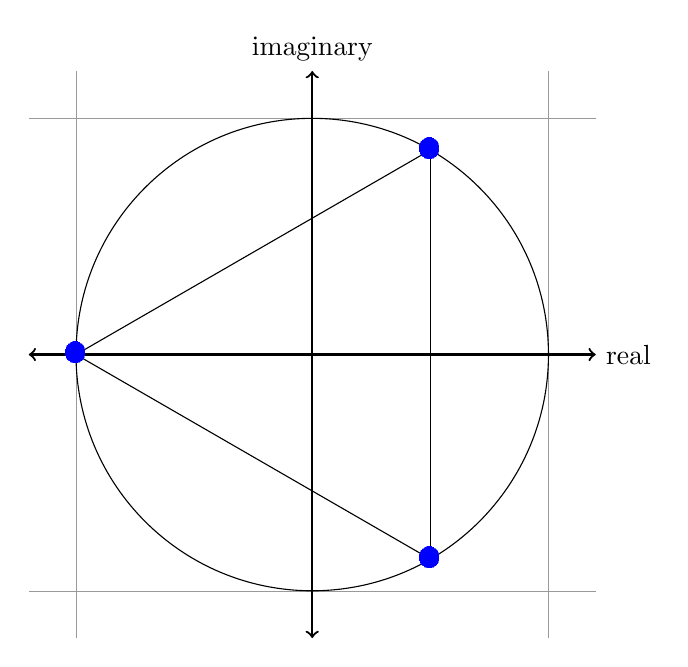
\begin{tikzpicture}[scale=3,domain=-2:2]
\draw[very thin,color=black!40] (-1.2,-1.2) grid (1.2,1.2);
\draw[thick,<->] (-1.2,0) -- (1.2,0) node[right] {real};
\draw[thick,<->] (0,-1.2) -- (0,1.2) node[above] {imaginary};
\draw[color=black] (0,0) circle (1);
\draw (-1,0) -- (0.5,0.866) ;
\draw (-1,0) -- (0.5,-0.866) ;
\draw (0.5,-0.866) -- (0.5,0.866) ;
\node[color=blue,scale=2] at (0.5,0.866) {\textbullet};
\node[color=blue,scale=2] at (-1,0) {\textbullet};
\node[color=blue,scale=2] at (0.5,-0.866) {\textbullet};
\end{tikzpicture}
\end{figure}

The principle root is $\frac{1}{2} + i \frac{\sqrt{3}}{2}$.

\section{Factoring Problem}
\begin{quote}
Factor $x^4+2$ over $\R$, $\Q$, and $\Co$.
\end{quote}

The roots of $x^4+2$ are the solutions to $x^4+2=0$.
\[ x^4+2=0 \]
\[ x^4= -2 \]
This has roots 
\[ 
z = \sqrt[4]{2} \exp\sq{ i \p{\frac{\pi}{4} + \frac{2k\pi}{4}} },
\qquad
k = 0,1,2,3
\]
Which reduces to
\[
z =\sqrt[4]{2} 
\p{ \cos\p{\frac{\pi+2k\pi}{4}} , \sin\p{\frac{\pi+2k\pi}{4}} }
\]

For $k=0$, this is $\sqrt[4]{2} (\cos(\pi/4),\sin(\pi/4)) = \sqrt[4]{2} (\sqrt{2}/2,\sqrt{2}/2) 
= 2^{1/4} \p{ 2^{-1/2} , 2^{-1/2} } = (2^{-1/4},2^{-1/4}) = \sqrt[4]{1/2} + i \sqrt[4]{1/2}$.

For $k=1$, this is $\sqrt[4]{2} (\cos(3\pi/4),\sin(3\pi/4)) 
= \sqrt[4]{2} (-\sqrt{2}/2,\sqrt{2}/2 )
= 2^{1/4} (-2^{-1/2} , 2^{-1/2} )
= (-2^{-1/4} , 2^{-1/4})
= -\sqrt[4]{1/2} + i \sqrt[4]{1/2}$.

By symmetry, for $k=2$, the root is $(-2^{-1/4},-2^{-1/4})$. Similarly, for $k=3$, the root is 
$(2^{-1/4},-2^{-1/4})$.

Thus, in $\Co[x]$, 
\begin{equation}\label{complex}
x^4+2 
= 
(x+2^{-1/4} + i 2^{-1/4})
(x-2^{-1/4} + i 2^{-1/4})
(x+2^{-1/4} - i 2^{-1/4})
(x-2^{-1/4} - i 2^{-1/4})
\end{equation}

To factor this in $\R[x]$, we must multiply the pairs of complex conjugate terms above, which yield
\[
(x+2^{-1/4} + i 2^{-1/4})
(x+2^{-1/4} - i 2^{-1/4})
=
x^2+2^{3/4} x + 2^{1/2}
\]
\[
(x-2^{-1/4} + i 2^{-1/4})
(x-2^{-1/4} - i 2^{-1/4})
=
x^2-2^{3/4} x + 2^{1/2}
\]
Hence,
\begin{equation}\label{real}
x^4+2
=
(x^2+2^{3/4} x + 2^{1/2})
(x^2-2^{3/4} x + 2^{1/2})
\end{equation}

Neither of these factor polynomials is in $\Q[x]$, however. Thus we conclude that 
\begin{equation}\label{rational}
x^4 + 2 = x^4 + 2
\end{equation}
is the only factorization of $x^4+2$ in $\Q[x]$.
\end{document}
